\chapter{Validation of pulse shape simulation}
\label{cha:psa}
The physics models \cite{miha, bart} for the drift of charge carriers and their measured input parameters \cite{miha, bart} alone are not enough to provide a realistic pulse shape simulation. While some input parameters are generic to germanium, others, like the impurity density and the detailed properties of the surface layers, are different for each detector. Thus the simulation has to be tuned for each individual detector or at least for a series of similar detectors. 

Several data samples were taken with the first GERDA Phase II prototype detector Siegfried I (see Sec.~\ref{sec:gerda:stat3}) operated in its test stand (see Sec.~\ref{sec:tt:comc}) to characterize the detector. The pulse shape simulation  was verified using these data. The results are presented in this chapter.

\section{Detector characterization measurements}
\label{sec:psa:char}
A detailed description of the characterization of Siegfried I is available in Ref.~\cite{Sie07}. Two data samples were used to verify the simulation:
\begin{description}
\item[Surface scanning:] The surfaces of segments 13, 14 and 15 (see Fig.~\ref{fig:ger:segm}) were scanned in $\phi$ (azimuth angle) using a 75~kBq $^{152}$Eu source inside a copper collimator with a length of 52~mm and a pin-hole diameter of 11~mm. The spot size on the detector surface was estimated to be $\approx 150$~mm$^{2}$. The distance between the collimator and the center of the detector was $\approx 85$~mm. The center of the collimator was pointed at $z = 0$ (see Fig.~\ref{fig:pss:coo}). 
The step size of the scan was  5$^{\circ}$ in segment 14 and 10$^{\circ}$ in segment 13 and 15. The uncertainty in $\phi$ is $\approx \Delta \phi=2.5^{\circ}$. In total 25~measurements were performed to cover 180$^{\circ}$ in azimuth. The pulses of the core and all segments were recorded. There were about $50\ 000$~events per measurement.
\item[Occupancy measurement:] A 60~kBq $^{60}$Co source was positioned about 15~cm above the center of Siegfried I (see Fig.~\ref{fig:ph:occ}). The energy deposits seen by each segment and the core were recorded.
\end{description}

The 122~keV $\gamma$ line of the $^{152}$Eu source used in the scan provided the events to study the drift of electrons. Because these low energy photons in average do not penetrate deeply into germanium and most likely deposit energy locally through the photoelectric effect (see Sec.~\ref{sec:det:gamma}), they create electron-hole pairs predominantly near the outer surface of the detector. The holes reach the outer surface almost immediately while the electrons have to drift through nearly the whole bulk of the detector until they reach the inner surface. Therefore, the pulse shapes are mainly determined by the drift of the electrons. 

To analyze the pulse shapes quantitatively the 10\%-30\% and 10\%-90\% risetimes of the core pulses were calculated. Figure~\ref{fig:psa:rt10} shows the average risetimes as a function of the azimuth angle $\phi$. The segment boundaries
are also indicated. Clear oscillation patterns can be seen in both cases. This confirms the longitudinal anisotropy of the drift velocity of electrons depending on the angle~$\phi$. The electrons need different times to drift nearly the same distance.\footnote{Strictly speaking, because of the bend of the drift trajectories the distances covered by electrons in different $\phi$ angles are sightly different from each other. However, this is a second-order effect. The difference of the risetimes is mainly caused by the different drift velocity along $r$ at different angles $\phi$.}
\begin{figure}[htbp]
\centering
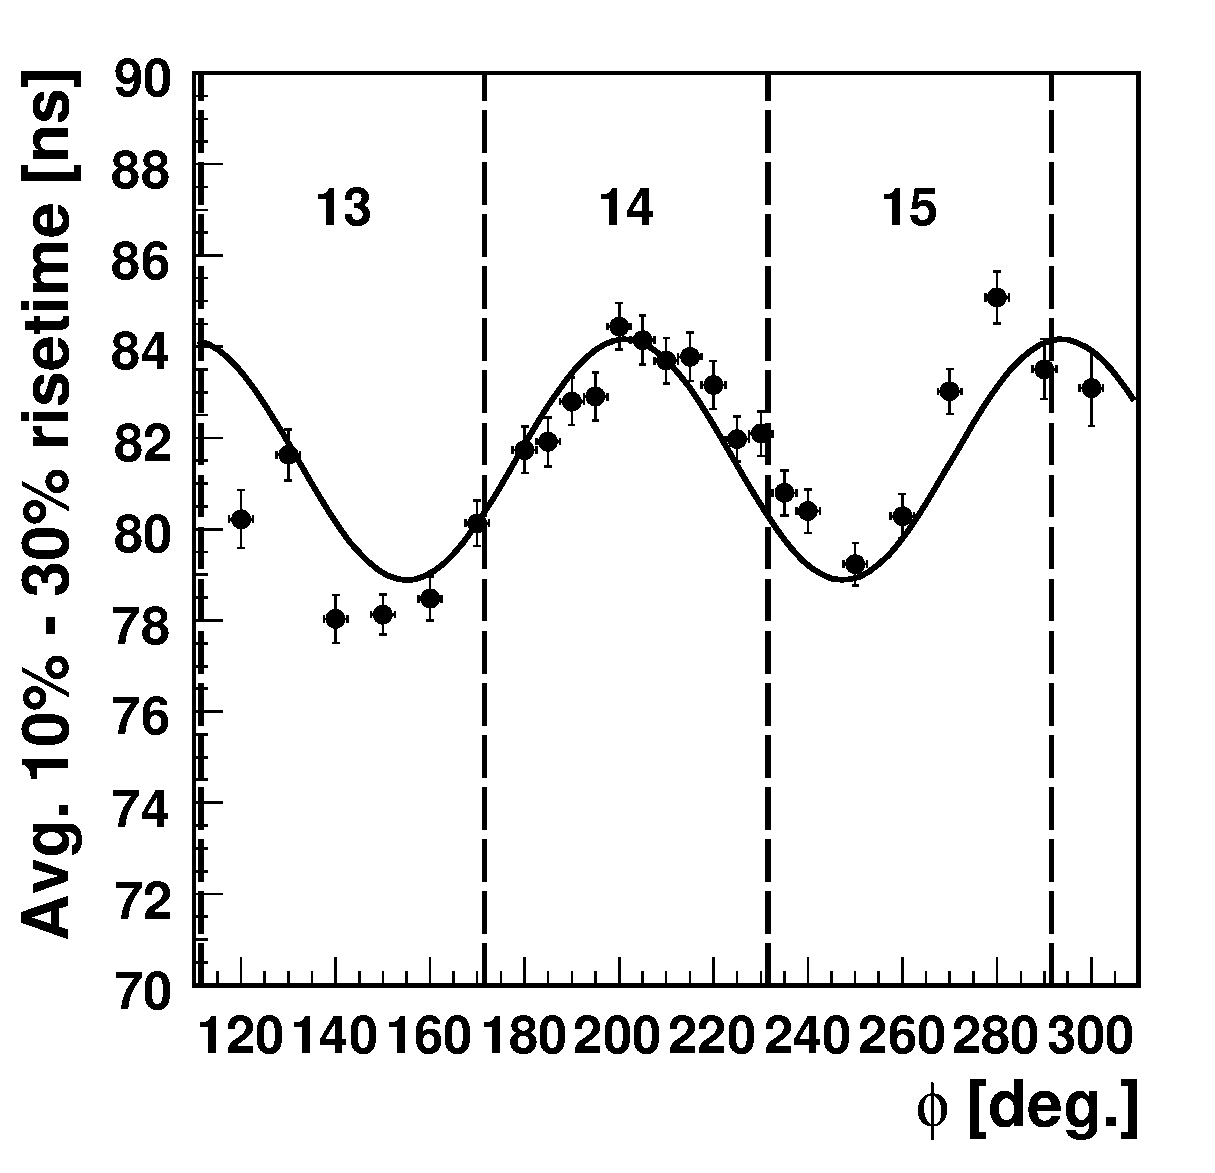
\includegraphics[width=0.45\textwidth]{phi_risetime1030}
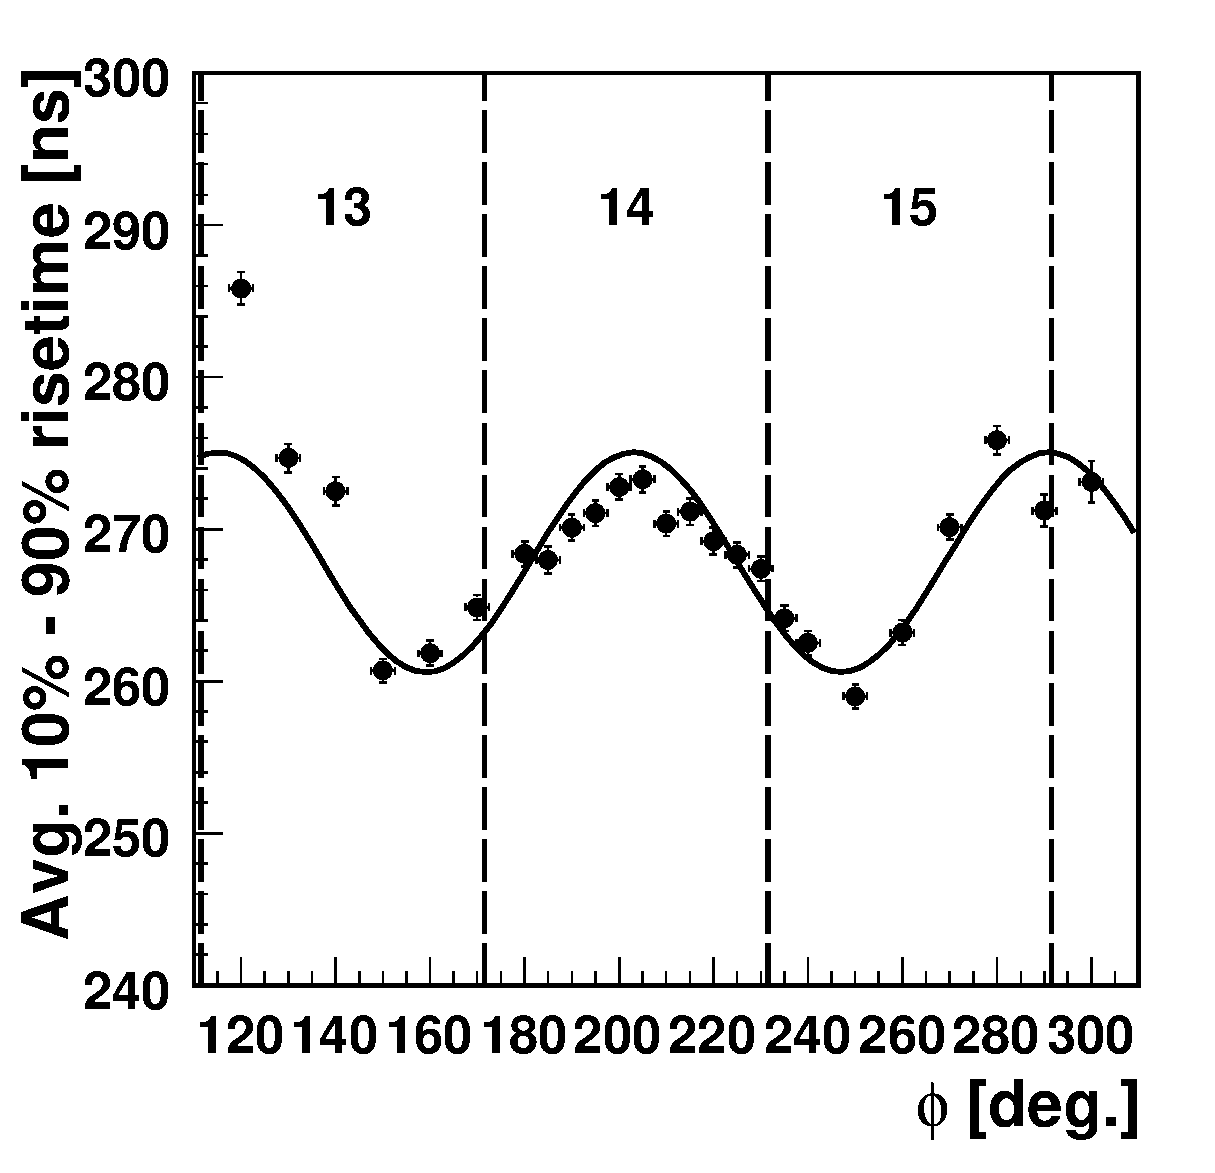
\includegraphics[width=0.45\textwidth]{phi_risetime1090}
\caption{Average 10\%-30\% (left) and 10\%-90\% (right) risetimes of the core pulses as a function of the azimuth angle $\phi$ (taken from Ref.~\cite{Sie07}).
The dashed lines indicate the segment boundaries.}
\label{fig:psa:rt10}
\end{figure}

Fits with a sine function (Fig.~\ref{fig:psa:rt10}) give periods of about 90$^{\circ}$ for the longitudinal anisotropy. This supports the model introduced in the previous chapter. The effect is illustrated in Fig.~\ref{fig:pss:trjs}. A direct comparison of the pulse shapes in data and simulation will follow
in the next section.

\section{Longitudinal anisotropy}
\label{sec:psa:lon}
Pulses induced in the core electrode by the drift of electrons starting at the outer surface of Siegfried I were simulated. The geometry, the operational voltage and the impurity density were implemented in the simulation according to the values listed in Table~\ref{tab:tt:detpar}. 

According to the model, electrons drift slowest along the $\langle 110 \rangle$ axes and ristimes reach their maxima. Thus, Figure~\ref{fig:psa:rt10} indicates that one of the $\langle 110 \rangle$ axes is nearly aligned with the right boundary of segment 15 at $\approx$\,290$^\circ$. This was implemented in the simulation. A decay time of 50~$\mu$s and a cut-off bandwidth of 37.5~MHz were implemented according to the specification of the electronics system. Electronic noise was not added to the pulse simulation to simplify
direct comparisons with individual pulses. Several parameters, \textit{i.e.} the \emph{Amplitude}, the \emph{Time offset} and the \emph{Time scaling factor} of the pulse, were introduced to fit the shape of a simulated to a measured pulse. The time offset shifts the pulse while the time scaling factor stretches or 
squeezes the pulse in time.

Figure~\ref{fig:psa:s2d} shows a randomly selected core pulse and the result of a fit with the simulated pulse along the $\langle 110 \rangle$ axis. The fit yields a time scaling factor of 0.81, indicating that the simulated pulse overestimates the pulse-length by $\approx 20\%$. Neverthless the $\chi^{2}$/NDF is excellent. In general a factor smaller than one is expected as the simulation reflects the maximal risetime.
\begin{figure}[htbp]
\centering
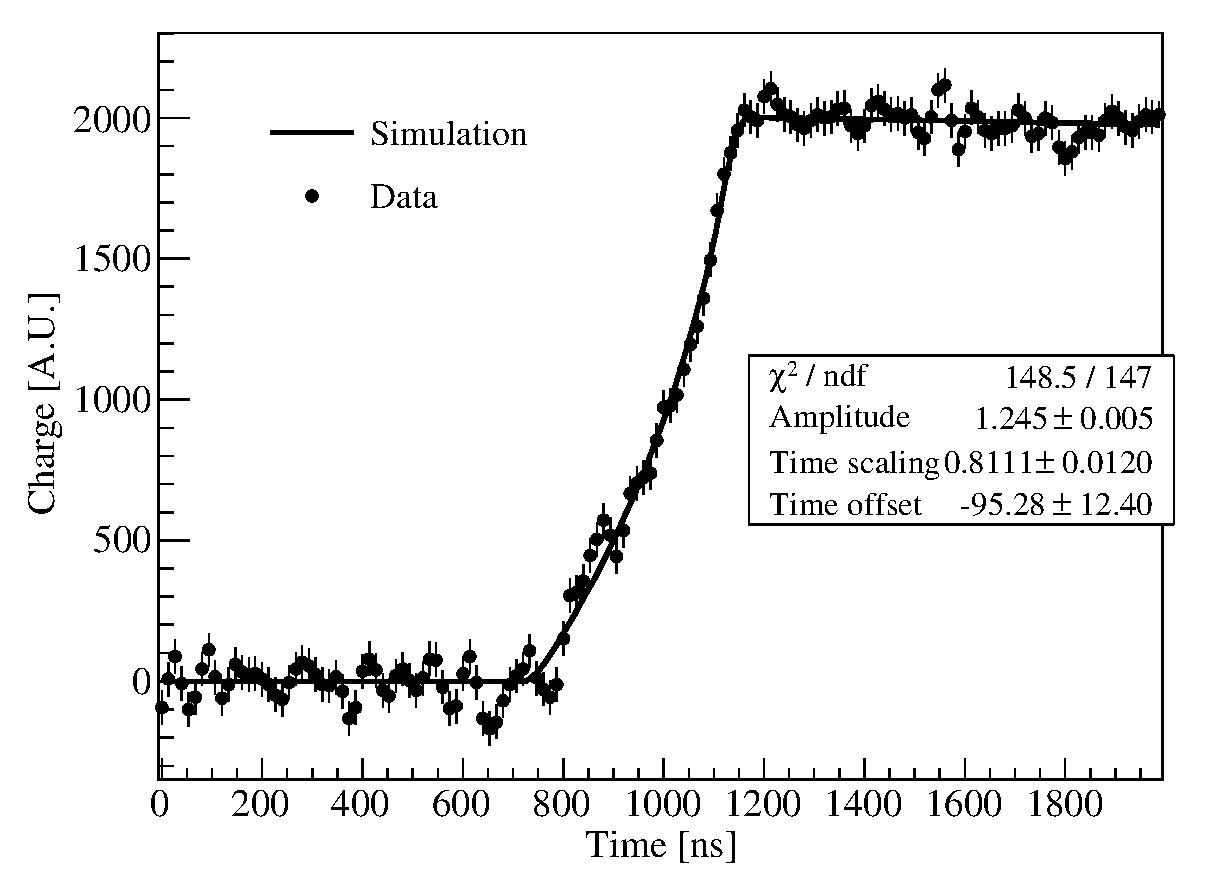
\includegraphics[width=0.6\textwidth]{PSs2d}
\caption{Fit of a simulated to a measured pulse. The dots represent the data and their error bars indicate the noise level.}
\label{fig:psa:s2d}
\end{figure}

A subset of pulses with fits were selected requiring
\begin{itemize}
\item $\chi^{2} < 200$ to eliminate very nosiy events,
\item $0.8 < Amplitude < 1.4$ to eliminate events misrecorded by the DAQ,
\item $Time offset > -300$~ns as very early pulses were not treated correctly by the DAQ.
\end{itemize}

\begin{figure}[htbp]
\centering
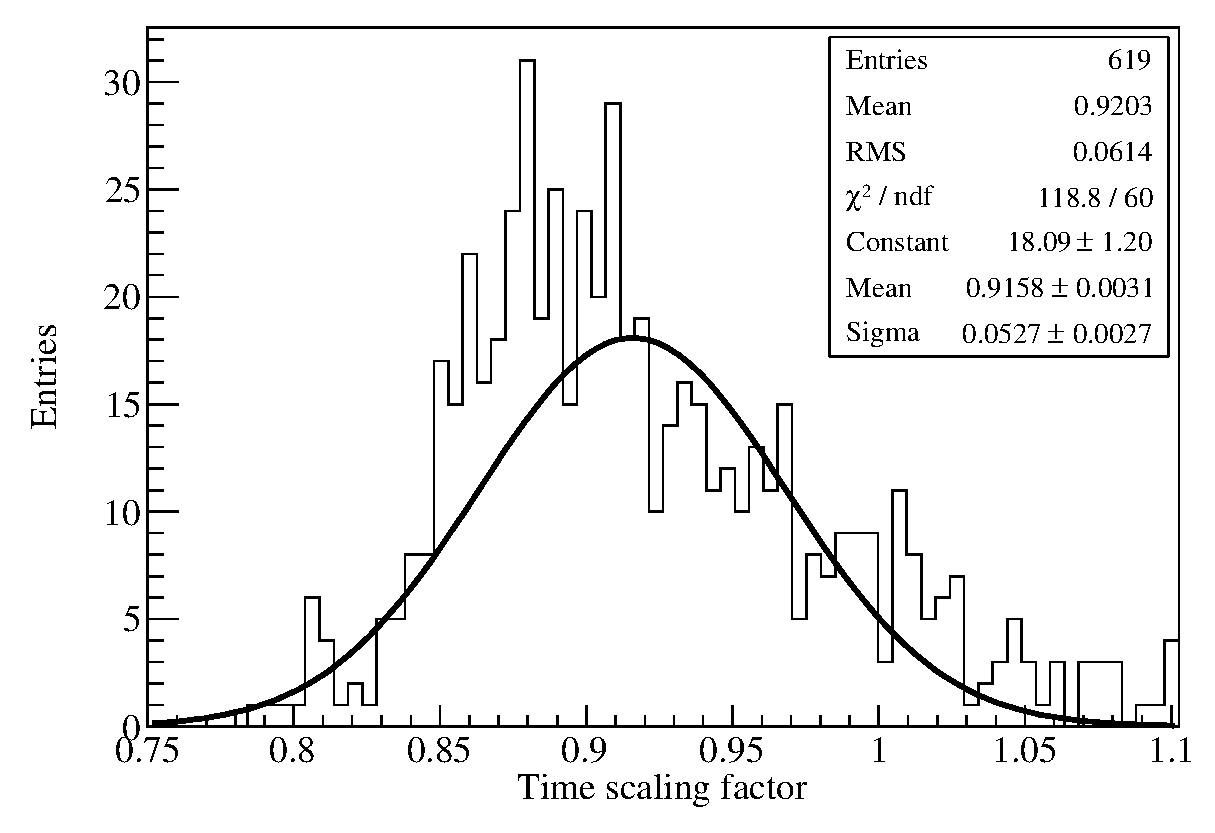
\includegraphics[width=0.5\textwidth]{tscale280}
\caption{Time scaling factors from the fits of the simulated to measured pulses taken at $\phi=280^{\circ}$.}
\label{fig:psa:ts280}
\end{figure}
The distributions of the time scaling factors for each scan position were fitted with a Gaussian function. Fig.~\ref{fig:psa:ts280} shows the distribution for $\phi = 280^{\circ}$. 
The scaling factor at $280^{\circ}$ should be close to one, if the the model would represent the detector perfectly. It is about 7\% lower.
However, the events in data do not start exactly at the outer surface.
The mean scaling factors obtained from the fits versus azimuth are displayed in Fig.~\ref{fig:psa:tsc}. The points were fitted with a sine wave plus a 1$^{st}$-order polynomial. The period of the sine wave was fixed to $90^{\circ}$. The shifted polynomial is shown as a baseline in Fig.~\ref{fig:psa:tsc}. The data is reasonably well described by the fit. However, the different values obtained for different instances of the $\langle 110 \rangle$ configuration indicate that the actual detector is more complex than assumed. One possible interpretation is that the impurity density given in Table~\ref{tab:tt:detpar} is an average density and in reality varies with the azimuthal angle $\phi$.

\begin{figure}[htbp]
\centering
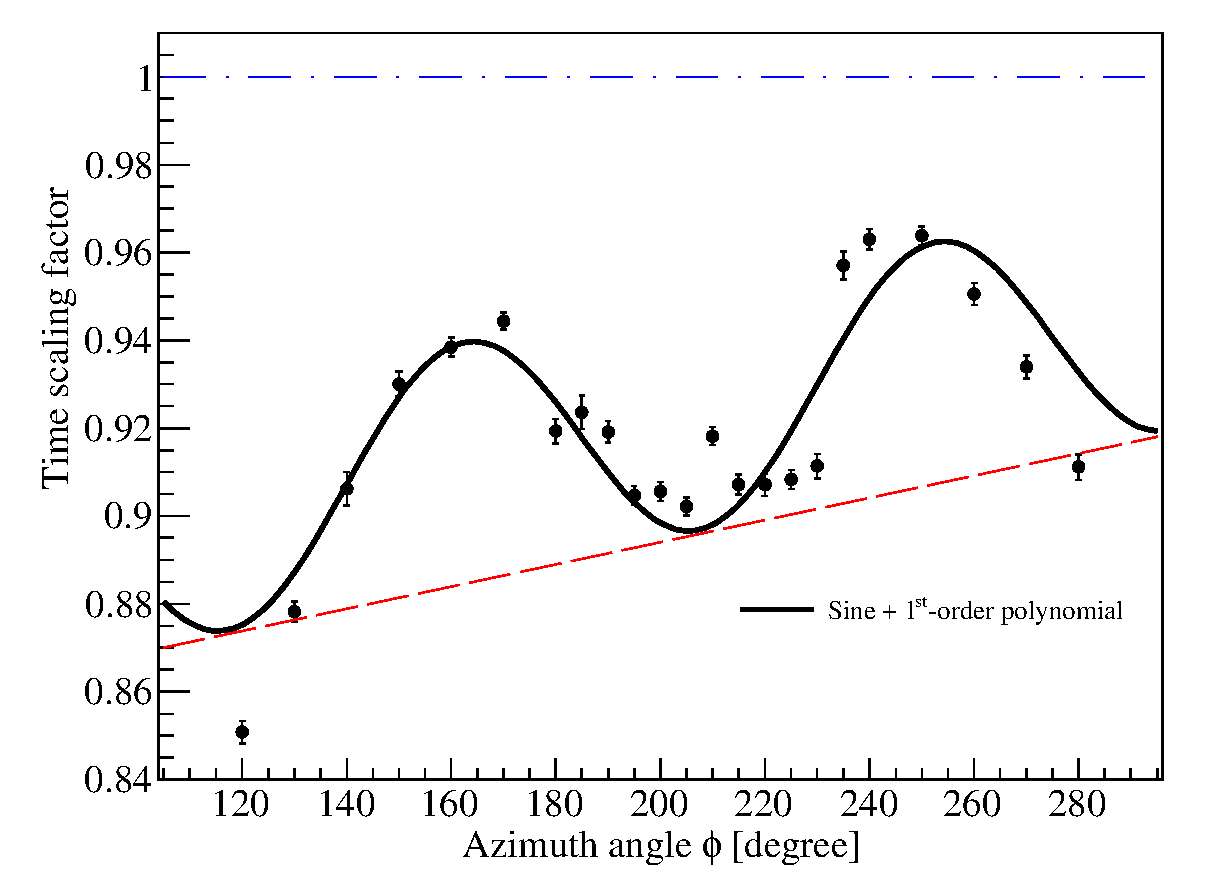
\includegraphics[width=0.6\textwidth]{tsc}
\caption{Mean time scaling factor (black dots) of a simulated $\langle 110 \rangle$ pulse versus azimuth. The solid line represents a fit with a sine wave plus a 1$^{st}$-order polynomial. The dashed line shows the shifted polynomial as a baseline.}
\label{fig:psa:tsc}
\end{figure}

The oscillation pattern expected and seen in Fig.~\ref{fig:psa:tsc} should disappear when the pulses are simulated for the indivual angular configuration of the the scan points. This was done and the result is depicted in fig.~\ref{fig:psa:tsl}. Also given is the shifted polynominal from the fit to the data in 
fig.~\ref{fig:psa:tsc} and a straight line fit to the points in fig.~\ref{fig:psa:tsl}. The two lines are very close confirming the predictions of the model for the angular dependence of the rise-time. The deviations from the fitted straight line are below 3\% and indicate that the real crystal is not as perfect as the simulated one. The overall shift relativ to one is in average about 10\% and can easily be corrected for. 

\begin{figure}[htbp]
\centering
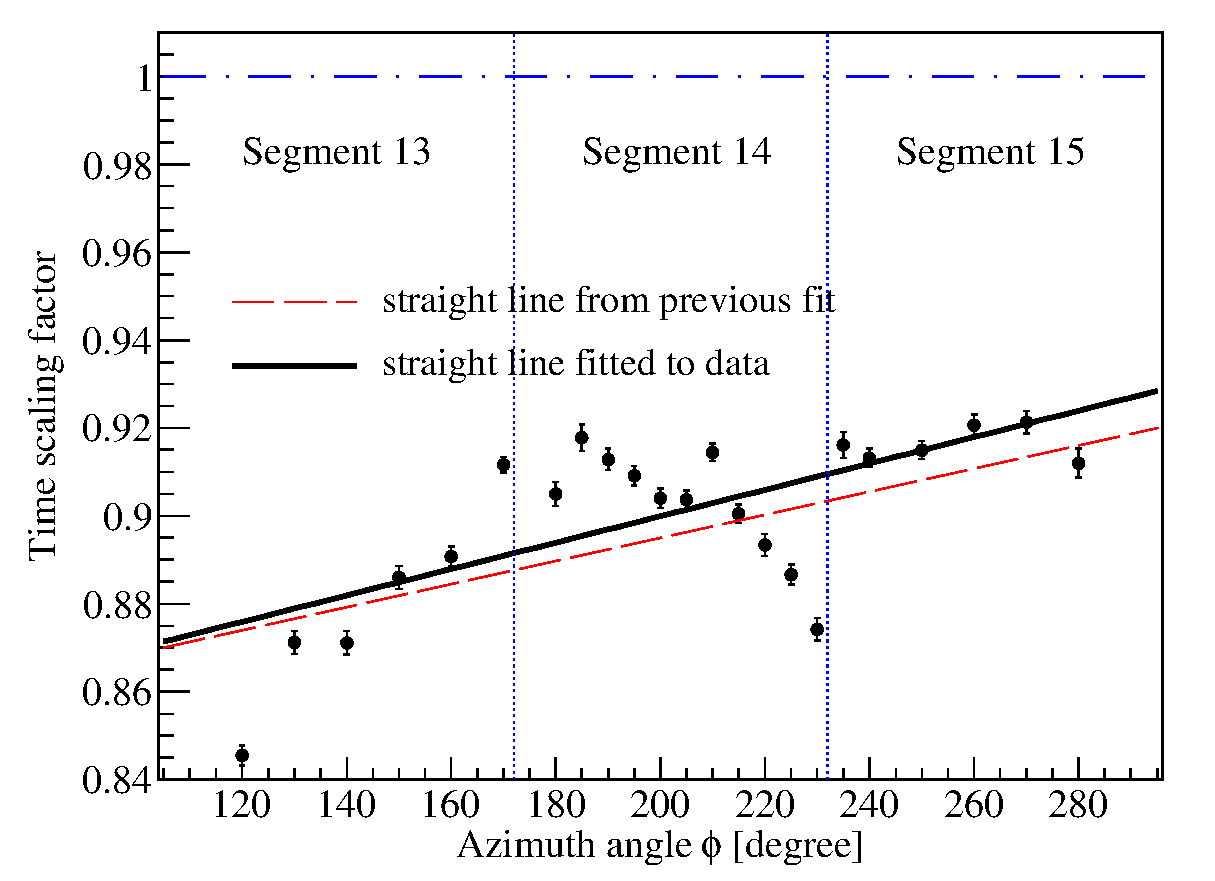
\includegraphics[width=0.6\textwidth]{tsline}
\caption{Mean time scaling factor (black dots) for pulses simulated for each angle individually against $\phi$. 
The result of a straight line fit is given as a solid line.
The shifted polynomial from Fig.~\ref{fig:psa:tsc} is overlaid for comparison. }
\label{fig:psa:tsl}
\end{figure}


\section{Transverse anisotropy}
\label{sec:psa:tra}
The transverse anisotropy of the drift leads to the bent drift trajectories shown in Fig.~\ref{fig:pss:trjs}. Consequently, the charge carriers created in one segment may drift into a neighboring segment. As a result, some segments always show a higher occupancy, because the trajectories are more likely to bend towards them. This effect was already shown in Fig.~\ref{fig:ph:mcb}. It is independent of the amount of energy deposited.

To verify quantitatively how well the effect can be described, $100\ 000$ hits with the same energy were homogeneously distributed in the middle 
layer of Siegfried I. The drift of holes was simulated for each location. If a trajectory ended on the outer surface of a given segment, its occupancy increased by one.

The predicted occupancies depend on the orientation of the crystal 
axes where the $\langle 110 \rangle$ axis is 
again used  as a reference. 
The resulting $\phi$-dependence of the occupancies 
was fitted to data with the orientation of the  $\langle 110 \rangle$ 
axis as a free parameter. The occupancies 
from the best fit are given 
in Fig.~\ref{fig:psa:focc}a. 
The direction of the $\langle 110 \rangle$ axis from 
the fit is only $4^\circ$ different from one of 
the segment boundaries. This is in good agreement 
with the result from the scan.

Figure~\ref{fig:psa:focc}b shows the $\chi^2$/dof versus$\phi_{110}$, 
the azimuthal difference between 
the orientation of the $\langle 110 \rangle$ axis and the segment boundary. 
Due to the crystal structure there is a $90^{\circ}$ degeneracy
in the $\chi^2$ distribution.  
As also reflected in Fig.~\ref{fig:psa:focc}a the $\chi^2$/NDF is not good. 
However, the minima in the $\chi^2$ distribution are very distinct,
allowing nevertheless a precise determination 
of the orientation of the crystal axes.

\begin{figure}[htbp]
\centering
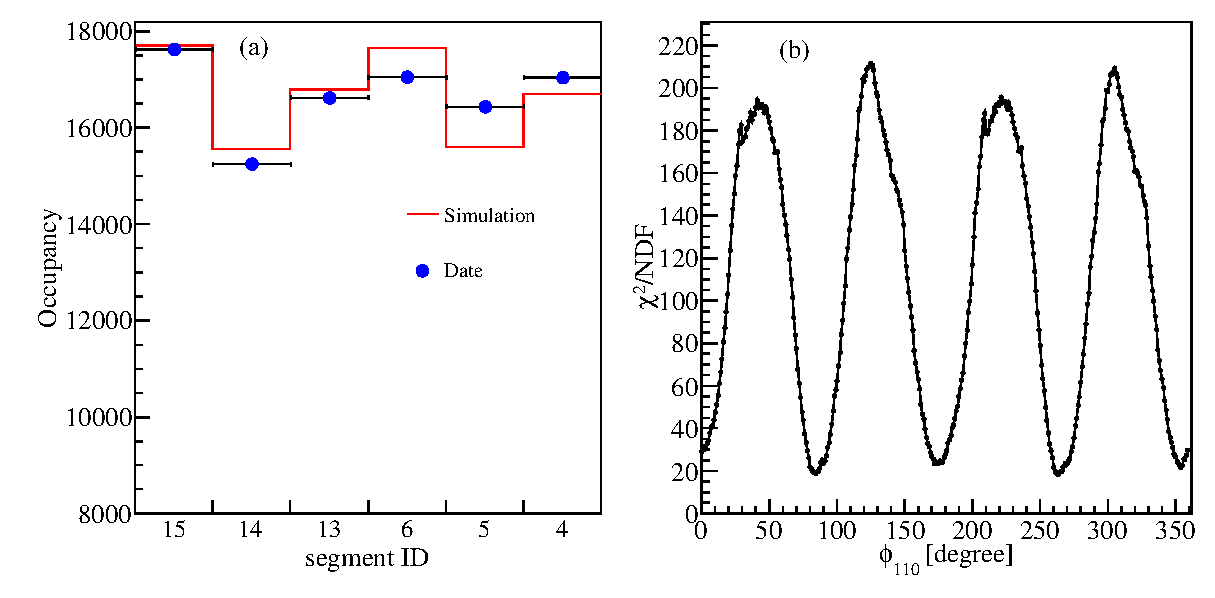
\includegraphics[width=0.9\textwidth]{fitocc}
\caption{(a) Occupancies of each segment (see Fig.~\ref{fig:ger:segm} for the segmentation scheme) for data (dots) and best fit simulation(histogram). (b) $\chi^{2}$/NDF of the fit described in the text versus $\phi_{110}$, the angle between the $\langle 110 \rangle$ axis and the segment boundary.}
\label{fig:psa:focc}
\end{figure}

While the overall behaviour of the data is well decribed, 
the precise differences in occupancy cannot be perfectly reproduced.
The segmentation and crystal axes orientations 
together have a $180^{\circ}$ degeneracy: if the segment 
boundaries or the crystal axes are rotated 
around the $z$-axis by $180^{\circ}$, 
the whole configuration does not change. 
This is refelected in the simulation which predicts the same pattern 
for segments 15, 14, and 13 and segments 6,5, and 4. 
The data, however, do not provide identical differences in occupancy. 
The first three segments show larger differences than the last three. 
One possible explanations is that the impurity density varies around $\phi$.


\section{Summary}
\label{sec:psa:sum}

The data confirm 
the longitudinal and transverse anisotropies inherent to 
the model of the drift of charges carriers used to simulate pulses 
in germanium detectors. 
The longitudinal anisotropy connected to the drift of electrons 
was seen in the dependence of the rise-time on the azimuthal angle, 
$\phi$, of the energy deposition. 
After an overall simple adjustment the simulation 
reproduces the risetimes within $\pm$3\%.

The transverse anisotropy connected to the drift of holes was observed 
as variations of the occupancy of segments 
located at different $\phi$. It was established 
that these variations can be used to 
determine the crystal orientation without a time 
consuming scan of the crystal.

%%% Local Variables:
%%% mode:latex
%%% TeX-master: "thesis"
%%% End:
